% Preamble
\documentclass[10pt,a4paper]{article}

% Packages
\usepackage[czech]{babel}
\usepackage[utf8]{inputenc}
\usepackage[T1]{fontenc}
\usepackage{float}
\usepackage{lmodern}
\usepackage[none]{hyphenat}
\usepackage[left=2cm, text={17cm, 24cm}, top=2cm]{geometry}
\usepackage{graphicx}
\usepackage{xcolor}
\usepackage{amsmath}
\usepackage{amssymb}
\usepackage{caption}
\usepackage{subcaption}
\usepackage{titlesec}
\usepackage{hyperref}
\usepackage{listings}
\usepackage{enumitem}
\usepackage{wasysym}
\usepackage{fancyhdr}
\usepackage{lastpage}
\usepackage{newpxtext}
\usepackage{longtable,ltcaption}
\usepackage{textgreek}
\usepackage{multirow}

\graphicspath{ {./img/} }

% \comment{}
\newcommand{\comment}[1]{}

% Document
\begin{document}

    % TITULNI STRANA
    \pagestyle{empty}
    \begin{titlepage}
        \begin{center}
            \large\normalsize{Vysoké učení technické v Brně\linebreak}
            \large\normalsize{Fakulta informačních technologií}

            \vfill
            
            \Large\textbf{Databázové systémy\linebreak}
            \Large\textbf{2021/2022}

            \vfill

            \LARGE\textbf{Zadání č. 33 – Lékarna\linebreak}

            \vfill
            \vfill
            \vfill


            \large{Marek Klofera (xklofe01), Tomáš Szabó (xszabo16) \hfill Brno, \today}
            
        \end{center}
    \end{titlepage}
    \pagestyle{plain}
    \newpage

    % OBSAH - SEKCE
    \tableofcontents
    \newpage

\section{Zadání}
        Vaším úkolem je vývoj IS lékárny. Lékárna vydává občanům léky jak na předpis, tak za hotové. U léků vydávaných na předpis může část ceny hradit zdravotní pojišťovna. Některé léky se vydávají pouze na předpis. Systém musí umožnit evidenci vydávaných léků, import příspěvků na léky od zdravotních pojišťoven (může se čas od času měnit), musí poskytovat export výkazů pro zdravotní pojišťovny a musí mít vazbu na skladové zásoby (vidět, zda požadovaný lék je na skladě). Léky jsou identifikovány číselným kódem či názvem.
        
    \newpage
        \subsection{ER diagram}
            \begin{figure}[H]
                \centering
                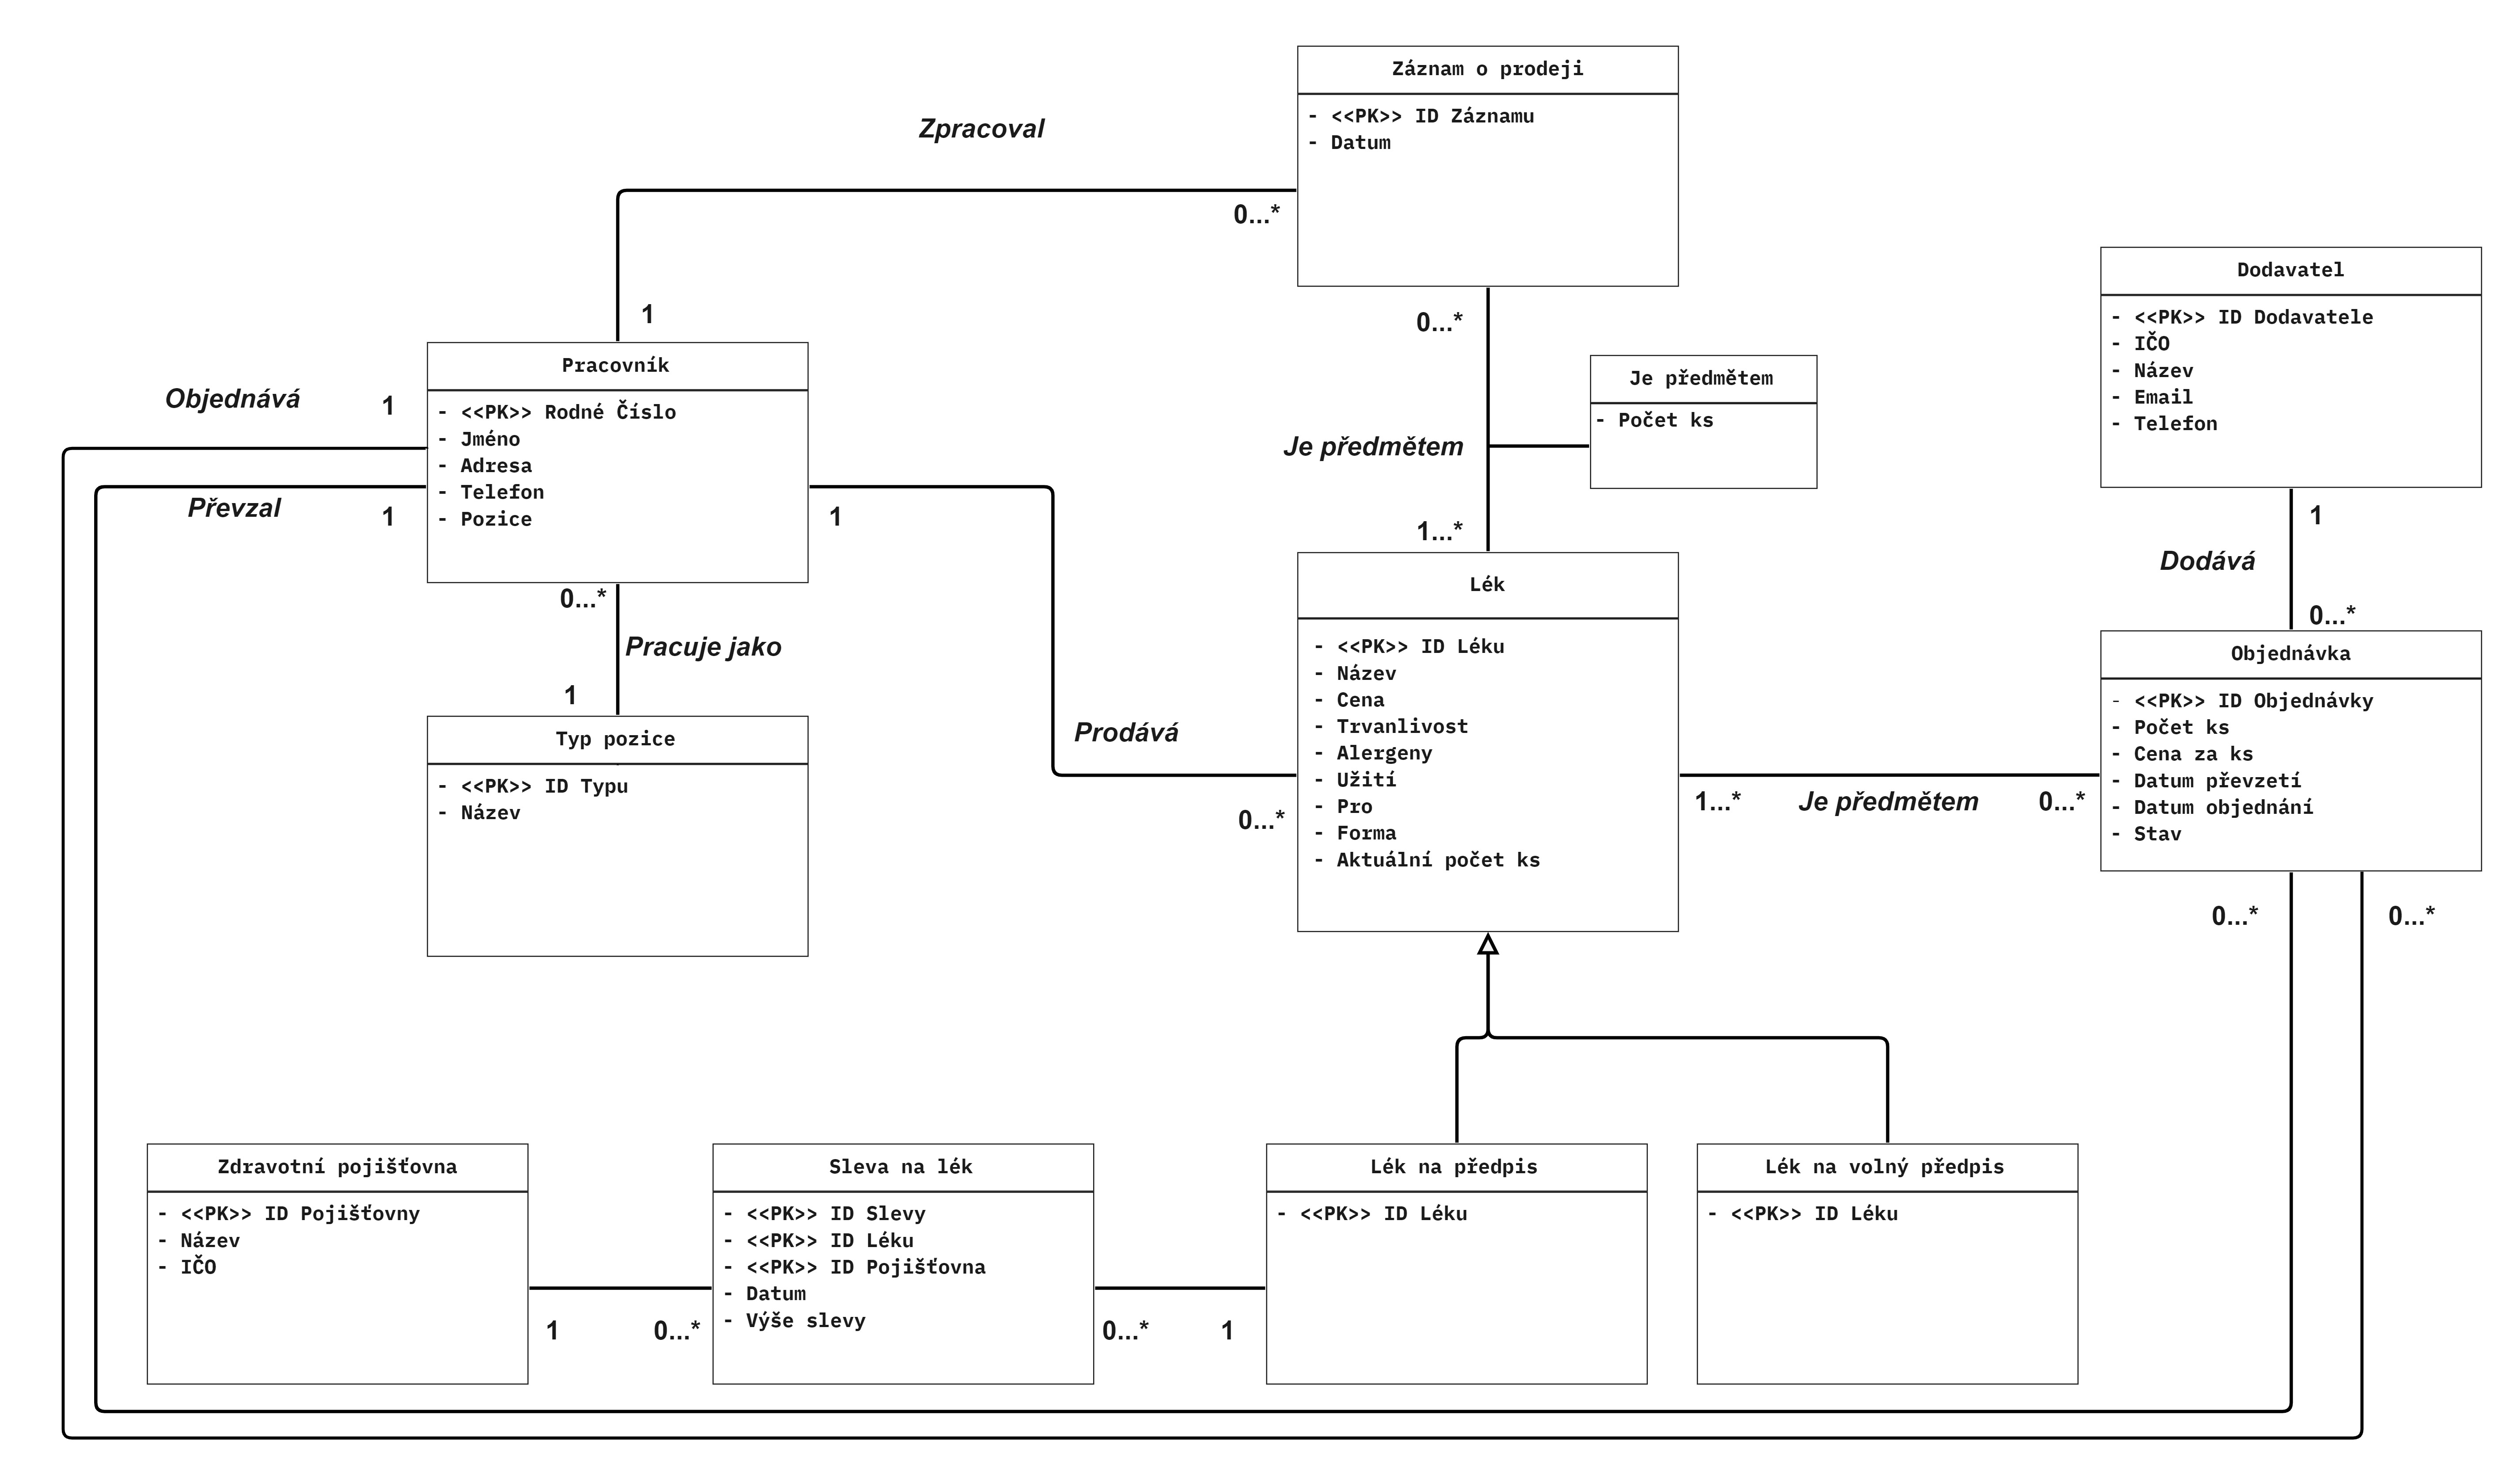
\includegraphics[scale=0.08]{img/ER.jpg}
                \label{fig:my_label}
            \end{figure}
            
        \subsection{Use Case diagram}
            \begin{figure}[H]
                \centering
                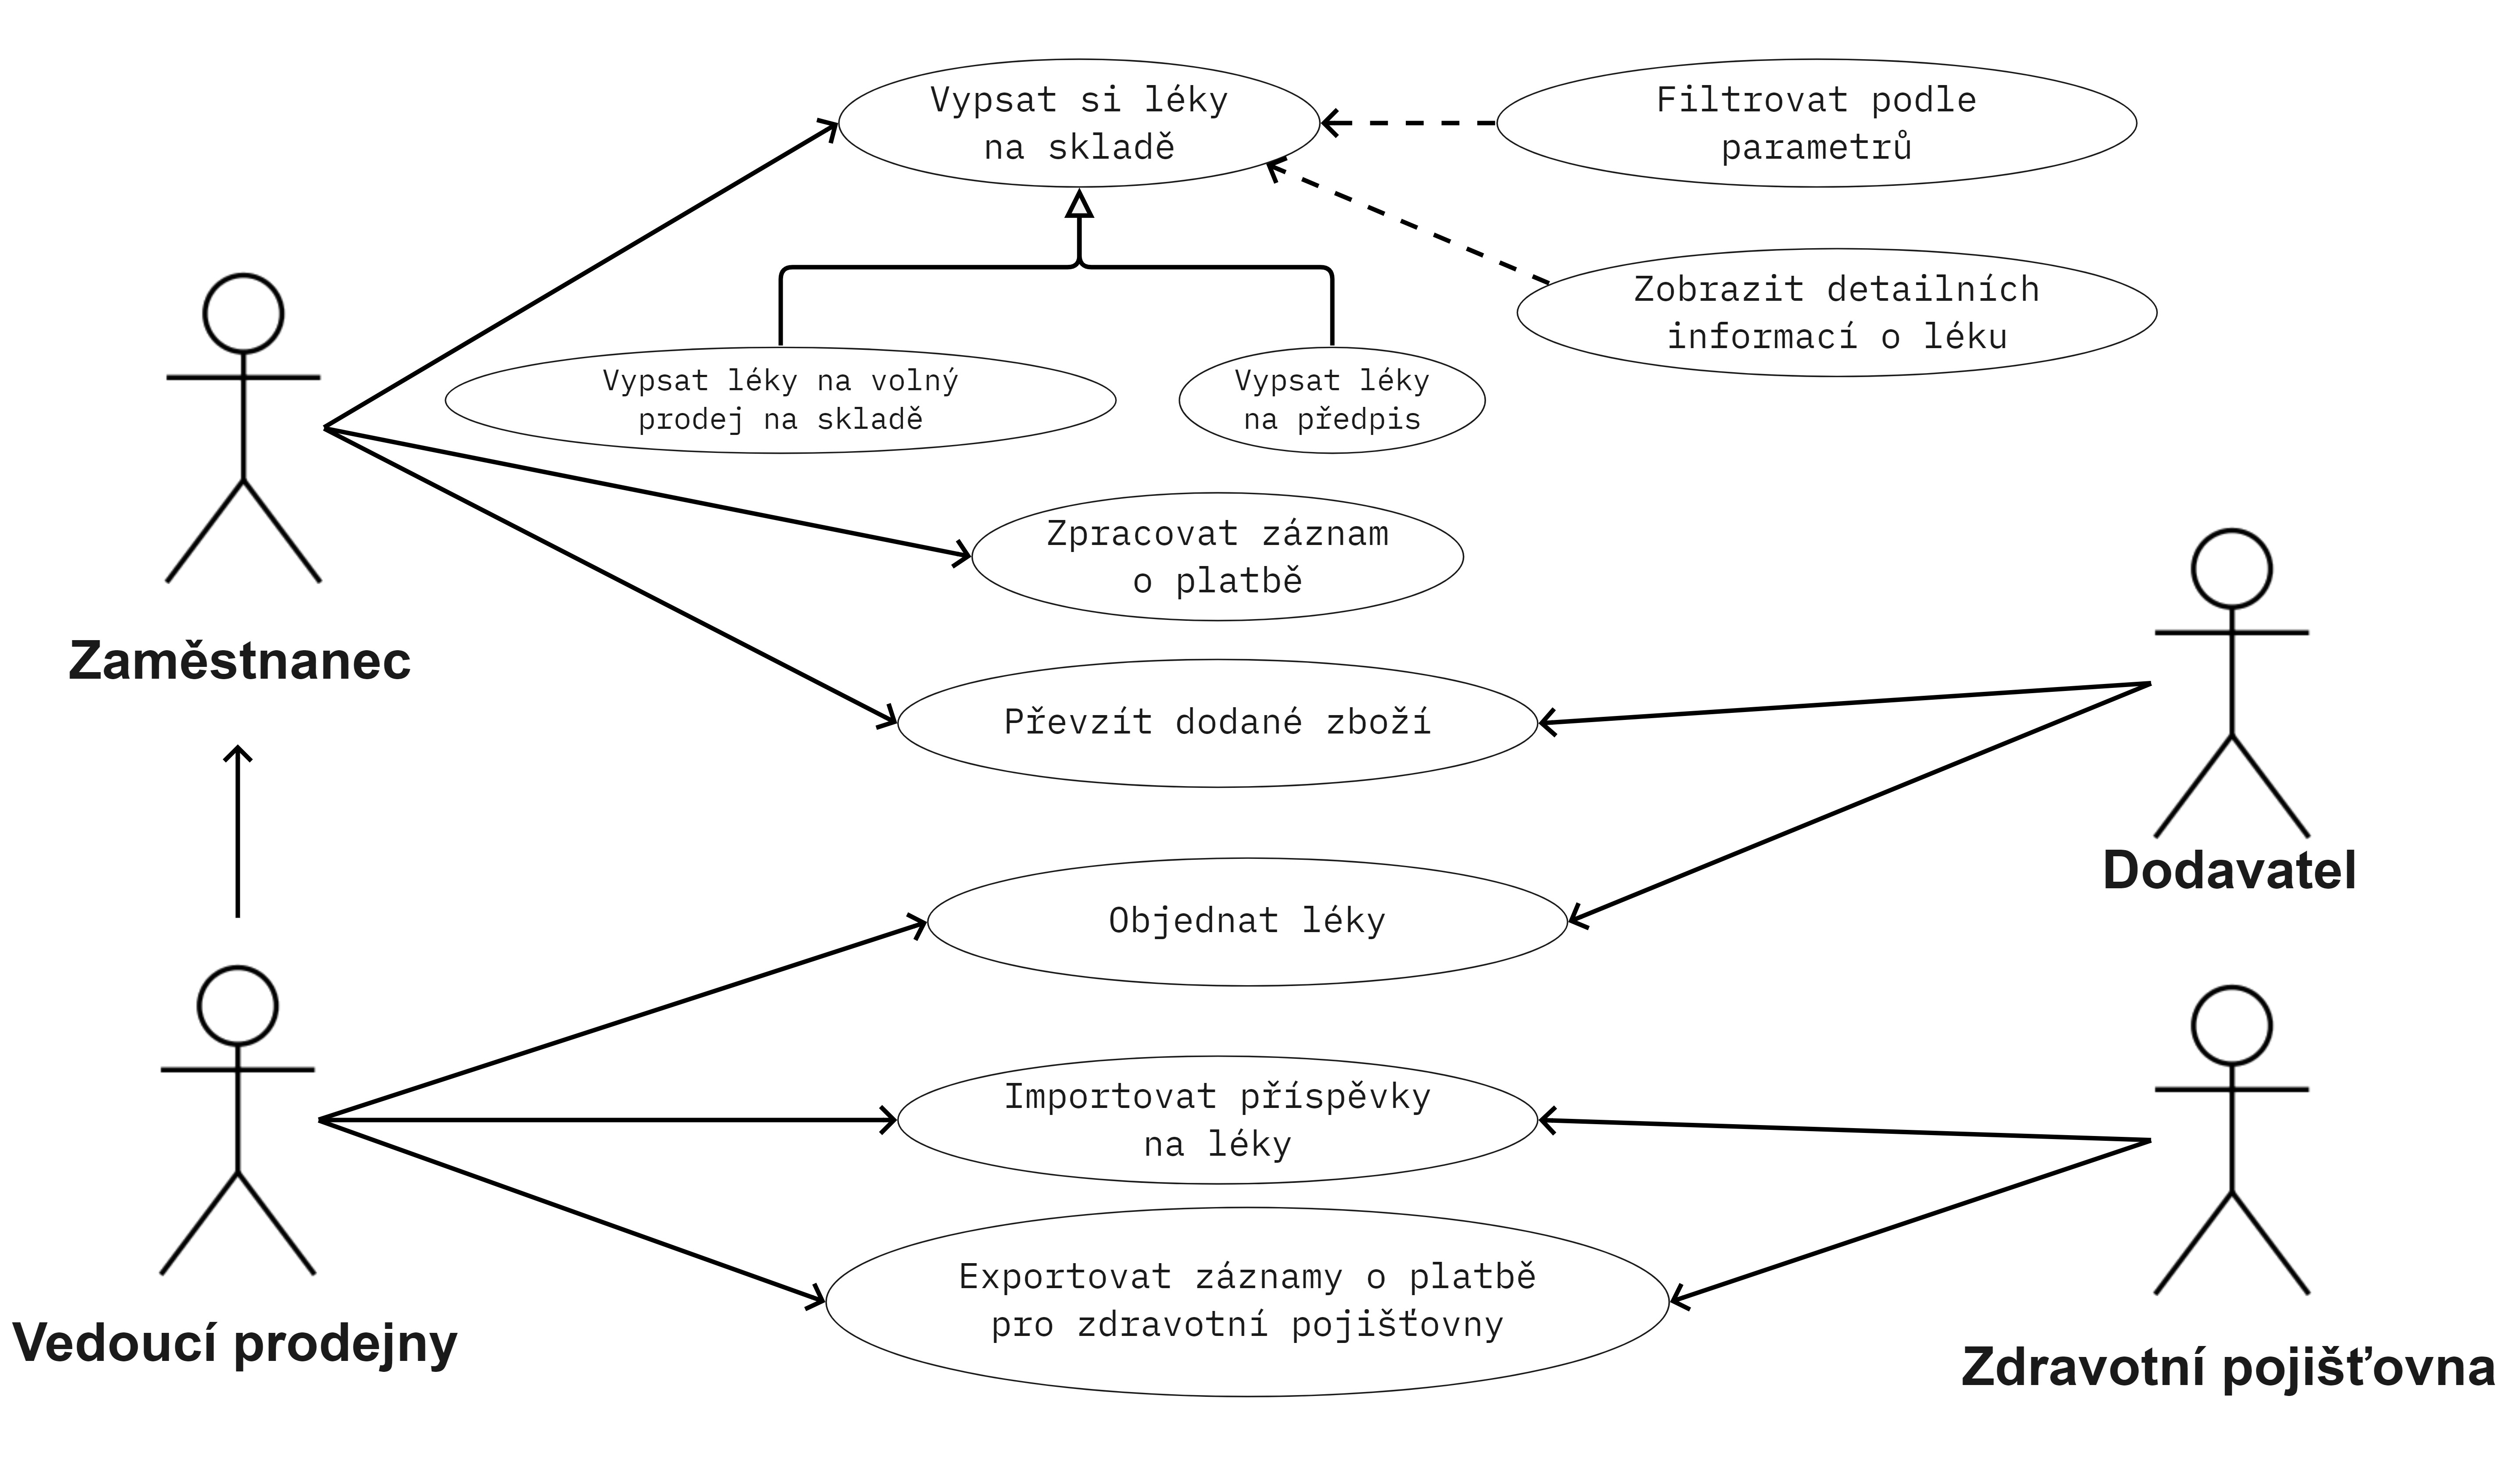
\includegraphics[scale=0.08]{img/useCase.jpg}
                \label{fig:my_label}
            \end{figure}
        
    
        \newpage
    
    \section{Trigger}
        \subsection{Navýšení počtu léků na skladě}
            \textit Při přijetí objednávky s léky se přičte patřičný počet léků do skladových zásob.
        
        \subsection{Snížení počtu léků na skladě}
            \textit Při prodeji některého z léků se vytvoří záznam o prodeji a trigger odečte patřičný počet léků ze skladových zásob. V případě, že je v záznamu o prodeji větší počet léků než počet léků na skladě léky se neodečítají a spustí se application error, který chybu ohlasí.
            
            Záznam o prodeji se nemaže, slouží k určení poptávky.
            
    \section{Procedure}
        \subsection{Přehled prodejů}
            \textit Procedura slouží k zjištění průměrného počtu prodaných léků na záznam o prodeji, v případě dělení 0 je tato chyba ohlášena na výstup.
            
         \subsection{Přehled léků s daným alergenem}
            \textit Procedura slouží k zjištění počtu léků s daným alergenem.
            
    \section{Explain Plan}
        \textit Explain plan ukazuje detail určitého příkazu. Byl použit již vytvořený SELECT z předchozí části projektu, který vrací částku s celkovým prodejem každého zaměstance.
        
        Po vytvoření indexu byl tento SELECT zrychlen skoro o polovinu jeho předchozího času.
        
    \section{Materialized view}
        \textit Slouží k uložení query infomací i v případě, že se tyto informace v databázi změní.
        
        V našem případě jsme si vytvořili pohled, který zobrazuje léky, které byly v minulosti prodány. Při změně názvu léku se tato změna neprojeví při opětovném volání pohledu.
        
    \section{Přístupová práva}
        \textit přidělení práv druhému členu týmu.
        
    \newpage
    \section{Závěr}
     \textit Všechny části čtvrté části projektu byli testovány a jejich správnost byla patřičně ověřena.
    
\end{document}